\documentclass[journal,twoside,web]{ieeecolor}
\usepackage{jsen}
\usepackage{cite}
\usepackage{amsmath,amssymb,amsfonts}
\usepackage{algorithmic}
\usepackage{graphicx}
\usepackage{textcomp}
\usepackage{wrapfig}
\def\BibTeX{{\rm B\kern-.05em{\sc i\kern-.025em b}\kern-.08em
    T\kern-.1667em\lower.7ex\hbox{E}\kern-.125emX}}
\markboth{\journalname, VOL. XX, NO. XX, XXXX 2017}
{Author \MakeLowercase{\textit{et al.}}: Preparation of Papers for IEEE TRANSACTIONS and JOURNALS (February 2017)}
\definecolor{abstractbg}{rgb}{0.89804,0.94510,0.83137}
\setlength{\fboxrule}{0pt}
\setlength{\fboxsep}{0pt}
\begin{document}
\title{Multiplex Detection with Multispectral Sensors and Machine Learning }
\author{First A. Author, \IEEEmembership{Fellow, IEEE}, Second B. Author, and Third C. Author, Jr., \IEEEmembership{Member, IEEE}
\thanks{This paragraph of the first footnote will contain the date on 
which you submitted your paper for review. It will also contain support 
information, including sponsor and financial support acknowledgment. For 
example, ``This work was supported in part by the U.S. Department of 
Commerce under Grant BS123456.'' }
\thanks{The next few paragraphs should contain 
the authors' current affiliations, including current address and e-mail. For 
example, F. A. Author is with the National Institute of Standards and 
Technology, Boulder, CO 80305 USA (e-mail: author@boulder.nist.gov). }
\thanks{S. B. Author, Jr., was with Rice University, Houston, TX 77005 USA. He is 
now with the Department of Physics, Colorado State University, Fort Collins, 
CO 80523 USA (e-mail: author@lamar.colostate.edu).}
\thanks{T. C. Author is with 
the Electrical Engineering Department, University of Colorado, Boulder, CO 
80309 USA, on leave from the National Research Institute for Metals, 
Tsukuba, Japan (e-mail: author@nrim.go.jp).}}

\IEEEtitleabstractindextext{%
\fcolorbox{abstractbg}{abstractbg}{%
\begin{minipage}{\textwidth}%
\begin{wrapfigure}[12]{r}{3in}%
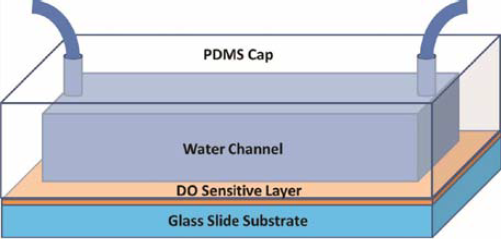
\includegraphics[width=3in]{jsenga.png}%
\end{wrapfigure}%
\begin{abstract}
These instructions give you guidelines for preparing papers for 
IEEE Transactions and Journals. Use this document as a template if you are 
using \LaTeX. Otherwise, use this document as an 
instruction set. The electronic file of your paper will be formatted further 
at IEEE. Paper titles should be written in uppercase and lowercase letters, 
not all uppercase. Avoid writing long formulas with subscripts in the title; 
short formulas that identify the elements are fine (e.g., "Nd--Fe--B"). Do 
not write ``(Invited)'' in the title. Full names of authors are preferred in 
the author field, but are not required. Put a space between authors' 
initials. The abstract must be a concise yet comprehensive reflection of 
what is in your article. In particular, the abstract must be self-contained, 
without abbreviations, footnotes, or references. It should be a microcosm of 
the full article. The abstract must be between 150--250 words. Be sure that 
you adhere to these limits; otherwise, you will need to edit your abstract 
accordingly. The abstract must be written as one paragraph, and should not 
contain displayed mathematical equations or tabular material. The abstract 
should include three or four different keywords or phrases, as this will 
help readers to find it. It is important to avoid over-repetition of such 
phrases as this can result in a page being rejected by search engines. 
Ensure that your abstract reads well and is grammatically correct.
\end{abstract}

\begin{IEEEkeywords}
Enter key words or phrases in alphabetical 
order, separated by commas. For a list of suggested keywords, send a blank 
e-mail to keywords@ieee.org or visit \underline
{http://www.ieee.org/organizations/pubs/ani\_prod/keywrd98.txt}
\end{IEEEkeywords}
\end{minipage}}}

\maketitle

\section{Introduction}
\label{sec:introduction}
\IEEEPARstart{T}{his} document is a template for \LaTeX. If you are 
reading a paper or PDF version of this document, please download the 
electronic file, trans\_jour.tex, from the IEEE Web site at \underline
{http://www.ieee.org/authortools/trans\_jour.tex} so you can use it to prepare your manuscript. If 
you would prefer to use LaTeX, download IEEE's LaTeX style and sample files 
from the same Web page. You can also explore using the Overleaf editor at 
\underline
{https://www.overleaf.com/blog/278-how-to-use-overleaf-with-}\discretionary{}{}{}\underline
{ieee-collabratec-your-quick-guide-to-getting-started\#.}\discretionary{}{}{}\underline{xsVp6tpPkrKM9}

If your paper is intended for a conference, please contact your conference 
editor concerning acceptable word processor formats for your particular 
conference. 

IEEE will do the final formatting of your paper. If your paper is intended 
for a conference, please observe the conference page limits. 



\subsection{Multiplex Applications of QDs}
Define abbreviations and acronyms the first time they are used in the text, 
even after they have already been defined in the abstract. Abbreviations 
such as IEEE, SI, ac, and dc do not have to be defined. Abbreviations that 
incorporate periods should not have spaces: write ``C.N.R.S.,'' not ``C. N. 
R. S.'' Do not use abbreviations in the title unless they are unavoidable 
(for example, ``IEEE'' in the title of this article).
\subsection{Multi-spectral sensor in bio-assays}
Define abbreviations and acronyms the first time they are used in the text, 
even after they have already been defined in the abstract. Abbreviations 
such as IEEE, SI, ac, and dc do not have to be defined. Abbreviations that 
incorporate periods should not have spaces: write ``C.N.R.S.,'' not ``C. N. 
R. S.'' Do not use abbreviations in the title unless they are unavoidable 
(for example, ``IEEE'' in the title of this article).

\subsection{Machine learning background}
I think here is where we discuss background on Multiplex QD predictions and the
benefit in using raspberry pi vs smart phone?


\section{Methods}
Use either SI (MKS) or CGS as primary units. (SI units are strongly 
encouraged.) English units may be used as secondary units (in parentheses). 
This applies to papers in data storage. For example, write ``15 
Gb/cm$^{2}$ (100 Gb/in$^{2})$.'' An exception is when 
English units are used as identifiers in trade, such as ``3\textonehalf-in 
disk drive.'' Avoid combining SI and CGS units, such as current in amperes 
and magnetic field in oersteds. This often leads to confusion because 
equations do not balance dimensionally. If you must use mixed units, clearly 
state the units for each quantity in an equation.

\subsection{Multispectral sensing system}


The SI unit for magnetic field strength $H$ is A/m. However, if you wish to use 
units of T, either refer to magnetic flux density $B$ or magnetic field 
strength symbolized as $\mu _{0}H$. Use the center dot to separate 
compound units, e.g., ``A$\cdot $m$^{2}$.''

\subsection{Set up for testing our sensing system}
The SI unit for magnetic field strength $H$ is A/m. However, if you wish to use 
units of T, either refer to magnetic flux density $B$ or magnetic field 
strength symbolized as $\mu _{0}H$. Use the center dot to separate 
compound units, e.g., ``A$\cdot $m$^{2}$.''


\subsection{Description of Machine learning algorithms}

We have used supervised machine learning to predict the QD concentration from the eight wavelength intensities. For each observation $x_i$ for $i = 1,2,..,n$ there is an associated response measurement $y_i$. The goal during training, is to approximate a mapping function from the input $x$ to the output $y$ variable, so that when given a new set of unknown input data, the algorithm can correctly predict the correct output variable.  To avoid potential overfitting of the data, we have used 10fold-cross validation scheme.

We have tried 5 distinct types of ML algorithms to predict the QD concentration. In this section we provide a shot description and key properties of each ML algorithm.
(following the style of Subhendu Pandit paper)

\subsubsection{Univariate Models}
{One possible appraoch to predict multiple QD types is to train a model for each emitter. During inference time we run both models in sequence. 


"Gaussian process regression is nonparametric (i.e. not limited by a functional form), so rather than calculating the probability distribution of parameters of a specific function, GPR calculates the probability distribution over all admissible functions that fit the data. However, similar to the above, we specify a prior (on the function space), calculate the posterior using the training data, and compute the predictive posterior distribution on our points of interest."

"Regression NN predict an output variable as a function of the inputs. The input features (independent variables) can be categorical or numeric types, however, for regression NN, we require a numeric dependent variable. If the output variable is a categorical variable (or binary) the ANN will function as a classifier"

" random forest is a meta estimator that fits a number of classifying decision trees on various sub-samples of the dataset and uses averaging to improve the predictive accuracy and control over-fitting. The sub-sample size is controlled with the max samples parameter if bootstrap=True (default), otherwise the whole dataset is used to build each tree"

" Support Vector Regression is a supervised learning algorithm that is used to predict discrete values. Support Vector Regression uses the same principle as the SVMs. The basic idea behind SVR is to find the best fit line. In SVR, the best fit line is the hyperplane that has the maximum number of points."

"Linear regression is a linear model, e.g. a model that assumes a linear relationship between the input variables (x) and the single output variable (y). More specifically, that y can be calculated from a linear combination of the input variables (x).

When there is a single input variable (x), the method is referred to as simple linear regression. When there are multiple input variables, literature from statistics often refers to the method as multiple linear regression."


}

\subsubsection{Multivariate  Models}
{Here we briefly discuss the extensions required to make some of the models multivariate  

}

\subsubsection{Frequentist vs Bayesian Models}
{here we discuss the key differences in assumptions and applications between bayesian methods and frequentist methods. 
Also discuss confidence intervals, and some considerations when comparing models.}


\subsection{Training Details}
Here we can discuss general training details. Epochs, libraries we used. 
and other compute details
\subsubsection{Hyper-parameter Optimization}
{Every algorithm attempted here has various hyper-parameters that affect the corresponding optimization process. 
These can have a significant difference in learning, so its important we employ a search to find optimal hyper-parameters. I think we can 
make a table in appendix showing optimal hyperparameters   }


\begin{figure*}[!t]
\centerline{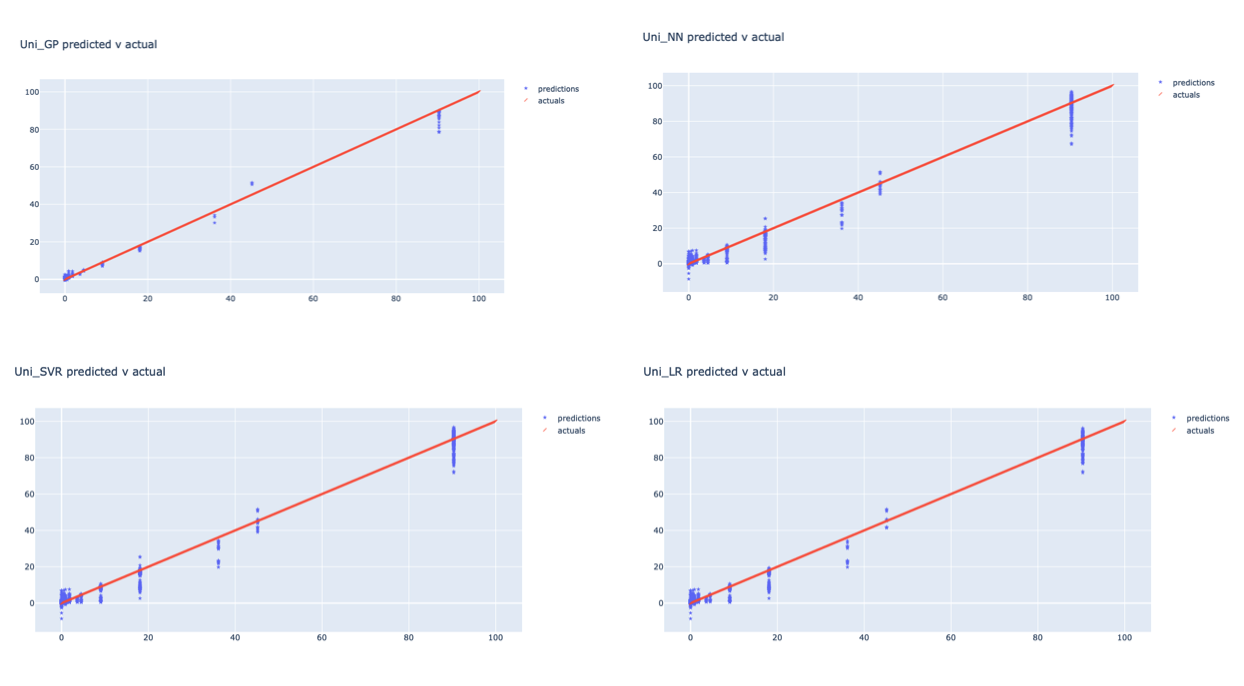
\includegraphics[width=15cm]{fig1.png}}
\caption{Magnetization as a function of applied field.
It is good practice to explain the significance of the figure in the caption.}
\label{fig1}
\end{figure*}




\begin{table}
\caption{Machine learning models}
\label{table}
\setlength{\tabcolsep}{3pt}
\begin{tabular}{|p{100pt}|p{45pt}|p{35pt}|p{50pt}|}
\hline
Model & 
Type& 
Accuracy\textsuperscript{*}   &
Trainable Parameters \\
\hline
Gaussian Process Reggression & 
Univariate& 
4.5   &
N/A\textsuperscript{**} \\
Linear Regression  & 
Univariate & 
4.5   &
1 \\
Bayesian Regression & 
Univariate & 
4.5   &
1 \\
Random Forest Regession & 
Univariate & 
4.5   &
1 \\
Neural Network & 
Univariate & 
4.5   &
1 \\
Neural Network & 
Multiivariate & 
4.5   &
1 \\
\hline
\multicolumn{4}{p{251pt}}{*Accuracy is measure of MSE for 10-fold Cross val. All models were tested using the same cross validation dataset breakdown. For univaraite models accuracy is the average between the two models}\\
\multicolumn{4}{p{251pt}}{**Bayesian methods are non-parametric and therefore have no trainable parameters}\\
\end{tabular}
\label{tab1}
\end{table}

\section{Results }


\subsection{Characterizing the limit of detection}

A conclusion section is not required. Although a conclusion may review the 
main points of the paper, do not replicate the abstract as the conclusion. A 
conclusion might elaborate on the importance of the work or suggest 
applications and extensions.

\subsection{Model Selection}

\subsubsection{Metrics}
{Figures that are composed of only black lines and shapes. These figures 
should have no shades or half-tones of gray, only black and white.}


Here we discuss cross validation accuracy and BIC, AIC criterial? 

\subsubsection{Confidence interval for Bayesian Methods}
{Figures that are composed of only black lines and shapes. These figures 
should have no shades or half-tones of gray, only black and white.}


\subsection{Making Predictions}

\subsubsection{Raspberry Pi Details}
{Figures that are composed of only black lines and shapes. These figures 
should have no shades or half-tones of gray, only black and white.}

\subsubsection{Confidence Intervals for retraining}
{Figures that are composed of only black lines and shapes. These figures 
should have no shades or half-tones of gray, only black and white.}


\section{Conclusion}
A conclusion section is not required. Although a conclusion may review the 
main points of the paper, do not replicate the abstract as the conclusion. A 
conclusion might elaborate on the importance of the work or suggest 
applications and extensions. A conclusion section is not required. Although a conclusion may review the 
main points of the paper, do not replicate the abstract as the conclusion. A 
conclusion might elaborate on the importance of the work or suggest 
applications and extensions. 

\appendices

Appendixes, if needed, appear before the acknowledgment.

\section*{Acknowledgment}

The preferred spelling of the word ``acknowledgment'' in American English is 
without an ``e'' after the ``g.'' Use the singular heading even if you have 
many acknowledgments. Avoid expressions such as ``One of us (S.B.A.) would 
like to thank $\ldots$ .'' Instead, write ``F. A. Author thanks $\ldots$ .'' In most 
cases, sponsor and financial support acknowledgments are placed in the 
unnumbered footnote on the first page, not here.

\section*{References and Footnotes}

\subsection{References}
References need not be cited in text. When they are, they appear on the 
line, in square brackets, inside the punctuation. Multiple references are 
each numbered with separate brackets. When citing a section in a book, 
please give the relevant page numbers. In text, refer simply to the 
reference number. Do not use ``Ref.'' or ``reference'' except at the 
beginning of a sentence: ``Reference \cite{b3} shows $\ldots$ .'' Please do not use 
automatic endnotes in \emph{Word}, rather, type the reference list at the end of the 
paper using the ``References'' style.

Reference numbers are set flush left and form a column of their own, hanging 
out beyond the body of the reference. The reference numbers are on the line, 
enclosed in square brackets. In all references, the given name of the author 
or editor is abbreviated to the initial only and precedes the last name. Use 
them all; use \emph{et al.} only if names are not given. Use commas around Jr., 
Sr., and III in names. Abbreviate conference titles. When citing IEEE 
transactions, provide the issue number, page range, volume number, year, 
and/or month if available. When referencing a patent, provide the day and 
the month of issue, or application. References may not include all 
information; please obtain and include relevant information. Do not combine 
references. There must be only one reference with each number. If there is a 
URL included with the print reference, it can be included at the end of the 
reference. 

Other than books, capitalize only the first word in a paper title, except 
for proper nouns and element symbols. For papers published in translation 
journals, please give the English citation first, followed by the original 
foreign-language citation See the end of this document for formats and 
examples of common references. For a complete discussion of references and 
their formats, see the IEEE style manual at
\underline{http://www.ieee.org/authortools}.

\subsection{Footnotes}
Number footnotes separately in superscript numbers.\footnote{It is recommended that footnotes be avoided (except for 
the unnumbered footnote with the receipt date on the first page). Instead, 
try to integrate the footnote information into the text.} Place the actual 
footnote at the bottom of the column in which it is cited; do not put 
footnotes in the reference list (endnotes). Use letters for table footnotes 
(see Table \ref{table}).

\section{Submitting Your Paper for Review}

\subsection{Final Stage}
When you submit your final version (after your paper has been accepted), 
print it in two-column format, including figures and tables. You must also 
send your final manuscript on a disk, via e-mail, or through a Web 
manuscript submission system as directed by the society contact. You may use 
\emph{Zip} for large files, or compress files using \emph{Compress, Pkzip, Stuffit,} or \emph{Gzip.} 

Also, send a sheet of paper or PDF with complete contact information for all 
authors. Include full mailing addresses, telephone numbers, fax numbers, and 
e-mail addresses. This information will be used to send each author a 
complimentary copy of the journal in which the paper appears. In addition, 
designate one author as the ``corresponding author.'' This is the author to 
whom proofs of the paper will be sent. Proofs are sent to the corresponding 
author only.

\subsection{Review Stage Using ScholarOne\textregistered\ Manuscripts}
Contributions to the Transactions, Journals, and Letters may be submitted 
electronically on IEEE's on-line manuscript submission and peer-review 
system, ScholarOne\textregistered\ Manuscripts. You can get a listing of the 
publications that participate in ScholarOne at 
\underline{http://www.ieee.org/publications\_standards/publications/}\discretionary{}{}{}\underline{authors/authors\_submission.html}.
First check if you have an existing account. If there is none, please create 
a new account. After logging in, go to your Author Center and click ``Submit 
First Draft of a New Manuscript.'' 

Along with other information, you will be asked to select the subject from a 
pull-down list. Depending on the journal, there are various steps to the 
submission process; you must complete all steps for a complete submission. 
At the end of each step you must click ``Save and Continue''; just uploading 
the paper is not sufficient. After the last step, you should see a 
confirmation that the submission is complete. You should also receive an 
e-mail confirmation. For inquiries regarding the submission of your paper on 
ScholarOne Manuscripts, please contact oprs-support@ieee.org or call +1 732 
465 5861.

ScholarOne Manuscripts will accept files for review in various formats. 
Please check the guidelines of the specific journal for which you plan to 
submit.

You will be asked to file an electronic copyright form immediately upon 
completing the submission process (authors are responsible for obtaining any 
security clearances). Failure to submit the electronic copyright could 
result in publishing delays later. You will also have the opportunity to 
designate your article as ``open access'' if you agree to pay the IEEE open 
access fee. 

\subsection{Final Stage Using ScholarOne Manuscripts}
Upon acceptance, you will receive an email with specific instructions 
regarding the submission of your final files. To avoid any delays in 
publication, please be sure to follow these instructions. Most journals 
require that final submissions be uploaded through ScholarOne Manuscripts, 
although some may still accept final submissions via email. Final 
submissions should include source files of your accepted manuscript, high 
quality graphic files, and a formatted pdf file. If you have any questions 
regarding the final submission process, please contact the administrative 
contact for the journal. 

In addition to this, upload a file with complete contact information for all 
authors. Include full mailing addresses, telephone numbers, fax numbers, and 
e-mail addresses. Designate the author who submitted the manuscript on 
ScholarOne Manuscripts as the ``corresponding author.'' This is the only 
author to whom proofs of the paper will be sent. 

\subsection{Copyright Form}
Authors must submit an electronic IEEE Copyright Form (eCF) upon submitting 
their final manuscript files. You can access the eCF system through your 
manuscript submission system or through the Author Gateway. You are 
responsible for obtaining any necessary approvals and/or security 
clearances. For additional information on intellectual property rights, 
visit the IEEE Intellectual Property Rights department web page at 
\underline{http://www.ieee.org/publications\_standards/publications/rights/}\discretionary{}{}{}\underline{index.html}. 

\section{IEEE Publishing Policy}
The general IEEE policy requires that authors should only submit original 
work that has neither appeared elsewhere for publication, nor is under 
review for another refereed publication. The submitting author must disclose 
all prior publication(s) and current submissions when submitting a 
manuscript. Do not publish ``preliminary'' data or results. The submitting 
author is responsible for obtaining agreement of all coauthors and any 
consent required from employers or sponsors before submitting an article. 
The IEEE Transactions and Journals Department strongly discourages courtesy 
authorship; it is the obligation of the authors to cite only relevant prior 
work.

The IEEE Transactions and Journals Department does not publish conference 
records or proceedings, but can publish articles related to conferences that 
have undergone rigorous peer review. Minimally, two reviews are required for 
every article submitted for peer review.

\section{Publication Principles}
The two types of contents of that are published are; 1) peer-reviewed and 2) 
archival. The Transactions and Journals Department publishes scholarly 
articles of archival value as well as tutorial expositions and critical 
reviews of classical subjects and topics of current interest. 

Authors should consider the following points:

\begin{enumerate}
\item Technical papers submitted for publication must advance the state of knowledge and must cite relevant prior work. 
\item The length of a submitted paper should be commensurate with the importance, or appropriate to the complexity, of the work. For example, an obvious extension of previously published work might not be appropriate for publication or might be adequately treated in just a few pages.
\item Authors must convince both peer reviewers and the editors of the scientific and technical merit of a paper; the standards of proof are higher when extraordinary or unexpected results are reported. 
\item Because replication is required for scientific progress, papers submitted for publication must provide sufficient information to allow readers to perform similar experiments or calculations and 
use the reported results. Although not everything need be disclosed, a paper 
must contain new, useable, and fully described information. For example, a 
specimen's chemical composition need not be reported if the main purpose of 
a paper is to introduce a new measurement technique. Authors should expect 
to be challenged by reviewers if the results are not supported by adequate 
data and critical details.
\item Papers that describe ongoing work or announce the latest technical achievement, which are suitable for presentation at a professional conference, may not be appropriate for publication.
\end{enumerate}

\section{Reference Examples}

\begin{itemize}

\item \emph{Basic format for books:}\\
J. K. Author, ``Title of chapter in the book,'' in \emph{Title of His Published Book, x}th ed. City of Publisher, (only U.S. State), Country: Abbrev. of Publisher, year, ch. $x$, sec. $x$, pp. \emph{xxx--xxx.}\\
See \cite{b1,b2}.

\item \emph{Basic format for periodicals:}\\
J. K. Author, ``Name of paper,'' \emph{Abbrev. Title of Periodical}, vol. \emph{x, no}. $x, $pp\emph{. xxx--xxx, }Abbrev. Month, year, DOI. 10.1109.\emph{XXX}.123456.\\
See \cite{b3}--\cite{b5}.

\item \emph{Basic format for reports:}\\
J. K. Author, ``Title of report,'' Abbrev. Name of Co., City of Co., Abbrev. State, Country, Rep. \emph{xxx}, year.\\
See \cite{b6,b7}.

\item \emph{Basic format for handbooks:}\\
\emph{Name of Manual/Handbook, x} ed., Abbrev. Name of Co., City of Co., Abbrev. State, Country, year, pp. \emph{xxx--xxx.}\\
See \cite{b8,b9}.

\item \emph{Basic format for books (when available online):}\\
J. K. Author, ``Title of chapter in the book,'' in \emph{Title of
Published Book}, $x$th ed. City of Publisher, State, Country: Abbrev.
of Publisher, year, ch. $x$, sec. $x$, pp. \emph{xxx--xxx}. [Online].
Available: \underline{http://www.web.com}\\
See \cite{b10}--\cite{b13}.

\item \emph{Basic format for journals (when available online):}\\
J. K. Author, ``Name of paper,'' \emph{Abbrev. Title of Periodical}, vol. $x$, no. $x$, pp. \emph{xxx--xxx}, Abbrev. Month, year. Accessed on: Month, Day, year, DOI: 10.1109.\emph{XXX}.123456, [Online].\\
See \cite{b14}--\cite{b16}.

\item \emph{Basic format for papers presented at conferences (when available online): }\\
J.K. Author. (year, month). Title. presented at abbrev. conference title. [Type of Medium]. Available: site/path/file\\
See \cite{b17}.

\item \emph{Basic format for reports and handbooks (when available online):}\\
J. K. Author. ``Title of report,'' Company. City, State, Country. Rep. no., (optional: vol./issue), Date. [Online] Available: site/path/file\\
See \cite{b18,b19}.

\item \emph{Basic format for computer programs and electronic documents (when available online): }\\
Legislative body. Number of Congress, Session. (year, month day). \emph{Number of bill or resolution}, \emph{Title}. [Type of medium]. Available: site/path/file\\
\textbf{\emph{NOTE: }ISO recommends that capitalization follow the accepted practice for the language or script in which the information is given.}\\
See \cite{b20}.

\item \emph{Basic format for patents (when available online):}\\
Name of the invention, by inventor's name. (year, month day). Patent Number [Type of medium]. Available: site/path/file\\
See \cite{b21}.

\item \emph{Basic format}\emph{for conference proceedings (published):}\\
J. K. Author, ``Title of paper,'' in \emph{Abbreviated Name of Conf.}, City of Conf., Abbrev. State (if given), Country, year, pp. \emph{xxxxxx.}\\
See \cite{b22}.

\item \emph{Example for papers presented at conferences (unpublished):}\\
See \cite{b23}.

\item \emph{Basic format for patents}$:$\\
J. K. Author, ``Title of patent,'' U.S. Patent \emph{x xxx xxx}, Abbrev. Month, day, year.\\
See \cite{b24}.

\item \emph{Basic format for theses (M.S.) and dissertations (Ph.D.):}
\begin{enumerate}
\item J. K. Author, ``Title of thesis,'' M.S. thesis, Abbrev. Dept., Abbrev. Univ., City of Univ., Abbrev. State, year.
\item J. K. Author, ``Title of dissertation,'' Ph.D. dissertation, Abbrev. Dept., Abbrev. Univ., City of Univ., Abbrev. State, year.
\end{enumerate}
See \cite{b25,b26}.

\item \emph{Basic format for the most common types of unpublished references:}
\begin{enumerate}
\item J. K. Author, private communication, Abbrev. Month, year.
\item J. K. Author, ``Title of paper,'' unpublished.
\item J. K. Author, ``Title of paper,'' to be published.
\end{enumerate}
See \cite{b27}--\cite{b29}.

\item \emph{Basic formats for standards:}
\begin{enumerate}
\item \emph{Title of Standard}, Standard number, date.
\item \emph{Title of Standard}, Standard number, Corporate author, location, date.
\end{enumerate}
See \cite{b30,b31}.

\item \emph{Article number in~reference examples:}\\
See \cite{b32,b33}.

\item \emph{Example when using et al.:}\\
See \cite{b34}.

\end{itemize}

\begin{thebibliography}{00}

\bibitem{b1} G. O. Young, ``Synthetic structure of industrial plastics,'' in \emph{Plastics,} 2\textsuperscript{nd} ed., vol. 3, J. Peters, Ed. New York, NY, USA: McGraw-Hill, 1964, pp. 15--64.

\bibitem{b2} W.-K. Chen, \emph{Linear Networks and Systems.} Belmont, CA, USA: Wadsworth, 1993, pp. 123--135.

\bibitem{b3} J. U. Duncombe, ``Infrared navigation---Part I: An assessment of feasibility,'' \emph{IEEE Trans. Electron Devices}, vol. ED-11, no. 1, pp. 34--39, Jan. 1959, 10.1109/TED.2016.2628402.

\bibitem{b4} E. P. Wigner, ``Theory of traveling-wave optical laser,'' \emph{Phys. Rev}., vol. 134, pp. A635--A646, Dec. 1965.

\bibitem{b5} E. H. Miller, ``A note on reflector arrays,'' \emph{IEEE Trans. Antennas Propagat}., to be published.

\bibitem{b6} E. E. Reber, R. L. Michell, and C. J. Carter, ``Oxygen absorption in the earth's atmosphere,'' Aerospace Corp., Los Angeles, CA, USA, Tech. Rep. TR-0200 (4230-46)-3, Nov. 1988.

\bibitem{b7} J. H. Davis and J. R. Cogdell, ``Calibration program for the 16-foot antenna,'' Elect. Eng. Res. Lab., Univ. Texas, Austin, TX, USA, Tech. Memo. NGL-006-69-3, Nov. 15, 1987.

\bibitem{b8} \emph{Transmission Systems for Communications}, 3\textsuperscript{rd} ed., Western Electric Co., Winston-Salem, NC, USA, 1985, pp. 44--60.

\bibitem{b9} \emph{Motorola Semiconductor Data Manual}, Motorola Semiconductor Products Inc., Phoenix, AZ, USA, 1989.

\bibitem{b10} G. O. Young, ``Synthetic structure of industrial
plastics,'' in Plastics, vol. 3, Polymers of Hexadromicon, J. Peters,
Ed., 2\textsuperscript{nd} ed. New York, NY, USA: McGraw-Hill, 1964, pp. 15-64.
[Online]. Available:
\underline{http://www.bookref.com}.

\bibitem{b11} \emph{The Founders' Constitution}, Philip B. Kurland
and Ralph Lerner, eds., Chicago, IL, USA: Univ. Chicago Press, 1987.
[Online]. Available: \underline{http://press-pubs.uchicago.edu/founders/}

\bibitem{b12} The Terahertz Wave eBook. ZOmega Terahertz Corp., 2014.
[Online]. Available:
\underline{http://dl.z-thz.com/eBook/zomega\_ebook\_pdf\_1206\_sr.pdf}. Accessed on: May 19, 2014.

\bibitem{b13} Philip B. Kurland and Ralph Lerner, eds., \emph{The
Founders' Constitution.} Chicago, IL, USA: Univ. of Chicago Press,
1987, Accessed on: Feb. 28, 2010, [Online] Available:
\underline{http://press-pubs.uchicago.edu/founders/}

\bibitem{b14} J. S. Turner, ``New directions in communications,'' \emph{IEEE J. Sel. Areas Commun}., vol. 13, no. 1, pp. 11-23, Jan. 1995.

\bibitem{b15} W. P. Risk, G. S. Kino, and H. J. Shaw, ``Fiber-optic frequency shifter using a surface acoustic wave incident at an oblique angle,'' \emph{Opt. Lett.}, vol. 11, no. 2, pp. 115--117, Feb. 1986.

\bibitem{b16} P. Kopyt \emph{et al., ``}Electric properties of graphene-based conductive layers from DC up to terahertz range,'' \emph{IEEE THz Sci. Technol.,} to be published. DOI: 10.1109/TTHZ.2016.2544142.

\bibitem{b17} PROCESS Corporation, Boston, MA, USA. Intranets:
Internet technologies deployed behind the firewall for corporate
productivity. Presented at INET96 Annual Meeting. [Online].
Available: \underline{http://home.process.com/Intranets/wp2.htp}

\bibitem{b18} R. J. Hijmans and J. van Etten, ``Raster: Geographic analysis and modeling with raster data,'' R Package Version 2.0-12, Jan. 12, 2012. [Online]. Available: \underline {http://CRAN.R-project.org/package=raster} 

\bibitem{b19} Teralyzer. Lytera UG, Kirchhain, Germany [Online].
Available:
\underline{http://www.lytera.de/Terahertz\_THz\_Spectroscopy.php?id=home}, Accessed on: Jun. 5, 2014

\bibitem{b20} U.S. House. 102\textsuperscript{nd} Congress, 1\textsuperscript{st} Session. (1991, Jan. 11). \emph{H. Con. Res. 1, Sense of the Congress on Approval of}  \emph{Military Action}. [Online]. Available: LEXIS Library: GENFED File: BILLS

\bibitem{b21} Musical toothbrush with mirror, by L.M.R. Brooks. (1992, May 19). Patent D 326 189 [Online]. Available: NEXIS Library: LEXPAT File: DES

\bibitem{b22} D. B. Payne and J. R. Stern, ``Wavelength-switched pas- sively coupled single-mode optical network,'' in \emph{Proc. IOOC-ECOC,} Boston, MA, USA, 1985, pp. 585--590.

\bibitem{b23} D. Ebehard and E. Voges, ``Digital single sideband detection for interferometric sensors,'' presented at the \emph{2\textsuperscript{nd} Int. Conf. Optical Fiber Sensors,} Stuttgart, Germany, Jan. 2-5, 1984.

\bibitem{b24} G. Brandli and M. Dick, ``Alternating current fed power supply,'' U.S. Patent 4 084 217, Nov. 4, 1978.

\bibitem{b25} J. O. Williams, ``Narrow-band analyzer,'' Ph.D. dissertation, Dept. Elect. Eng., Harvard Univ., Cambridge, MA, USA, 1993.

\bibitem{b26} N. Kawasaki, ``Parametric study of thermal and chemical nonequilibrium nozzle flow,'' M.S. thesis, Dept. Electron. Eng., Osaka Univ., Osaka, Japan, 1993.

\bibitem{b27} A. Harrison, private communication, May 1995.

\bibitem{b28} B. Smith, ``An approach to graphs of linear forms,'' unpublished.

\bibitem{b29} A. Brahms, ``Representation error for real numbers in binary computer arithmetic,'' IEEE Computer Group Repository, Paper R-67-85.

\bibitem{b30} IEEE Criteria for Class IE Electric Systems, IEEE Standard 308, 1969.

\bibitem{b31} Letter Symbols for Quantities, ANSI Standard Y10.5-1968.

\bibitem{b32} R. Fardel, M. Nagel, F. Nuesch, T. Lippert, and A. Wokaun, ``Fabrication of organic light emitting diode pixels by laser-assisted forward transfer,'' \emph{Appl. Phys. Lett.}, vol. 91, no. 6, Aug. 2007, Art. no. 061103.~

\bibitem{b33} J. Zhang and N. Tansu, ``Optical gain and laser characteristics of InGaN quantum wells on ternary InGaN substrates,'' \emph{IEEE Photon. J.}, vol. 5, no. 2, Apr. 2013, Art. no. 2600111

\bibitem{b34} S. Azodolmolky~\emph{et al.}, Experimental demonstration of an impairment aware network planning and operation tool for transparent/translucent optical networks,''~\emph{J. Lightw. Technol.}, vol. 29, no. 4, pp. 439--448, Sep. 2011.

\end{thebibliography}

\begin{IEEEbiography}[{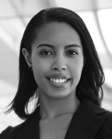
\includegraphics[width=1in,height=1.25in,clip,keepaspectratio]{a1.png}}]{First A. Author} (M'76--SM'81--F'87) and all authors may include 
biographies. Biographies are often not included in conference-related
papers. This author became a Member (M) of IEEE in 1976, a Senior
Member (SM) in 1981, and a Fellow (F) in 1987. The first paragraph may
contain a place and/or date of birth (list place, then date). Next,
the author's educational background is listed. The degrees should be
listed with type of degree in what field, which institution, city,
state, and country, and year the degree was earned. The author's major
field of study should be lower-cased. 

The second paragraph uses the pronoun of the person (he or she) and not the 
author's last name. It lists military and work experience, including summer 
and fellowship jobs. Job titles are capitalized. The current job must have a 
location; previous positions may be listed 
without one. Information concerning previous publications may be included. 
Try not to list more than three books or published articles. The format for 
listing publishers of a book within the biography is: title of book 
(publisher name, year) similar to a reference. Current and previous research 
interests end the paragraph. The third paragraph begins with the author's 
title and last name (e.g., Dr.\ Smith, Prof.\ Jones, Mr.\ Kajor, Ms.\ Hunter). 
List any memberships in professional societies other than the IEEE. Finally, 
list any awards and work for IEEE committees and publications. If a 
photograph is provided, it should be of good quality, and 
professional-looking. Following are two examples of an author's biography.
\end{IEEEbiography}

\begin{IEEEbiography}[{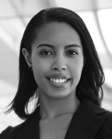
\includegraphics[width=1in,height=1.25in,clip,keepaspectratio]{a2.png}}]{Second B. Author} was born in Greenwich Village, New York, NY, USA in 
1977. He received the B.S. and M.S. degrees in aerospace engineering from 
the University of Virginia, Charlottesville, in 2001 and the Ph.D. degree in 
mechanical engineering from Drexel University, Philadelphia, PA, in 2008.

From 2001 to 2004, he was a Research Assistant with the Princeton Plasma 
Physics Laboratory. Since 2009, he has been an Assistant Professor with the 
Mechanical Engineering Department, Texas A{\&}M University, College Station. 
He is the author of three books, more than 150 articles, and more than 70 
inventions. His research interests include high-pressure and high-density 
nonthermal plasma discharge processes and applications, microscale plasma 
discharges, discharges in liquids, spectroscopic diagnostics, plasma 
propulsion, and innovation plasma applications. He is an Associate Editor of 
the journal \emph{Earth, Moon, Planets}, and holds two patents. 

Dr. Author was a recipient of the International Association of Geomagnetism 
and Aeronomy Young Scientist Award for Excellence in 2008, and the IEEE 
Electromagnetic Compatibility Society Best Symposium Paper Award in 2011. 
\end{IEEEbiography}

\begin{IEEEbiography}[{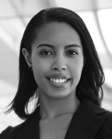
\includegraphics[width=1in,height=1.25in,clip,keepaspectratio]{a3.png}}]{Third C. Author, Jr.} (M'87) received the B.S. degree in mechanical 
engineering from National Chung Cheng University, Chiayi, Taiwan, in 2004 
and the M.S. degree in mechanical engineering from National Tsing Hua 
University, Hsinchu, Taiwan, in 2006. He is currently pursuing the Ph.D. 
degree in mechanical engineering at Texas A{\&}M University, College 
Station, TX, USA.

From 2008 to 2009, he was a Research Assistant with the Institute of 
Physics, Academia Sinica, Tapei, Taiwan. His research interest includes the 
development of surface processing and biological/medical treatment 
techniques using nonthermal atmospheric pressure plasmas, fundamental study 
of plasma sources, and fabrication of micro- or nanostructured surfaces. 

Mr. Author's awards and honors include the Frew Fellowship (Australian 
Academy of Science), the I. I. Rabi Prize (APS), the European Frequency and 
Time Forum Award, the Carl Zeiss Research Award, the William F. Meggers 
Award and the Adolph Lomb Medal (OSA).
\end{IEEEbiography}

\end{document}
